\documentclass[twoside,11pt]{report}

% Any additional packages needed should be included after jmlr2e.
% Note that jmlr2e.sty includes epsfig, amssymb, natbib and graphicx,
% and defines many common macros, such as 'proof' and 'example'.
%
% It also sets the bibliographystyle to plainnat; for more information on
% natbib citation styles, see the natbib documentation, a copy of which
% is archived at http://www.jmlr.org/format/natbib.pdf

\usepackage{jmlr2e}
% \usepackage[utf8]{inputenc}%
% \usepackage{tikz}
% \usepackage{cfr-lm}%
\usepackage[T1]{fontenc}%
\usepackage{physics}
\usepackage{amsmath}
% \usepackage{amssymb}
% \usepackage{graphicx}
% \usepackage[margin=3cm]{geometry}
% \usepackage{changepage}
\usepackage{fontspec}
\usepackage{minted}
\usepackage{tcolorbox}
\usepackage{lmodern}
\usepackage{xcolor}
\usepackage{lettrine}
% \usepackage{fontawesome}
\usemintedstyle{perldoc}
\hypersetup{colorlinks=false, pdfborder={0 0 0},  }
\usepackage{fancyhdr}
\usepackage{wrapfig}
\usepackage{adjustbox}
\usepackage{tikz}
% \usepackage{listofitems} % for \readlist to create arrays
\usepackage{caption}
\usepackage[toc,page,header]{appendix}


\newtcbox{\codebox}[1][black]{on line, arc=2pt,colback=#1!10!white,colframe=white, before upper={\rule[-3pt]{0pt}{10pt}},boxrule=1pt, boxsep=0pt,left=2pt,right=2pt,top=1pt,bottom=.5pt}
\newtcbox{\deloppg}[1][black]{on line, arc=2pt,colback=#1!10!white,colframe=white, before upper={\rule[-2pt]{0pt}{0pt}},boxrule=0pt, boxsep=0pt,left=.49\linewidth,right=.49\linewidth,top=4pt,bottom=3pt}


\newcommand\blfootnote[1]{ \begingroup \renewcommand\thefootnote{}\footnote{#1} \addtocounter{footnote}{-1} \endgroup }
% \definecolor{antwhite}{HTML}{323333}
\newcommand{\code}[3][]{\codebox{\mintinline[#1]{#2}{#3}}}



% \setmainfont{FreeSans}
% \setmainfont{SF Pro Display}
% \setmainfont{IBM Plex Sans}
% \setmainfont{TeX Gyre Heros}
% \setmainfont{Inter}
% \setmainfont{Iosevka Quasi}
% \setmainfont{DM Sans}

% \setmonofont{Iosevka Custom Extended}
% \setmonofont{JetBrainsMono Nerd Font}
\setmonofont[Scale=MatchLowercase]{DM Mono}





% Definitions of handy macros can go here

\newcommand{\dataset}{{\cal D}}
\newcommand{\fracpartial}[2]{\frac{\partial #1}{\partial  #2}}

\newtcolorbox[blend into=tables]{mytable}[2][]{float=htb, halign=center,  title={#2}, every float=\centering, #1}
% Heading arguments are {volume}{year}{pages}{submitted}{published}{author-full-names}

% \jmlrheading{1}{2000}{1-48}{4/00}{10/00}{https://github.com/bragewiseth/MachineLearningProjects}

% Short headings should be running head and authors last names

\ShortHeadings{\url{https://github.com/bragewiseth/MachineLearningProjects}}{\url{https://github.com/bragewiseth/MachineLearningProjects}}
\firstpageno{1}



\title{{Solving the Wave Equation with Neural Networks}}
\author{\name Brage W. \email bragewi@ifi.uio.no\\
    \name Felix C. H.  \email felixch@ifi.uio.no \\
\name Eirik B. J. \email eiribja@ifi.uio.no}
\date{\today}											% Date
\makeatletter






% \date{\today}

\usepackage{hyperref}
\begin{document}

%%%%%%%%%%%%%%%%%%%%%%%%%%%%%%%%%%%%%%%%%%%%%%%%%%%%%%%%%%%%%%%%%%%%%%%%%%%%%%%%%%%%%%%%%

\begin{titlepage}
    \centering
    \vspace*{0.5 cm}
    
\includegraphics[scale = 0.70]{uio.jpg}\\[0.2 cm]	% University Logo
    \textsc{\LARGE University of Oslo}\\[2.0 cm]	    % University Name
    \textsc{\Large FYS-STK3155}\\[0.5 cm]				% Course Code
    \rule{\linewidth}{0.2 mm} \\[0.4 cm]
    { \huge \bfseries \@title}\\
    \rule{\linewidth}{0.2 mm} \\[1.5 cm]

    \begin{minipage}{0.4\textwidth}
        \begin{flushleft} \normalsize
            Brage Wiseth\\
            Felix Cameren Heyerdahl\\
            Eirik Bjørnson Jahr\\
        \end{flushleft}
    \end{minipage}~
    \begin{minipage}{0.4\textwidth}
        \begin{flushright} \normalsize
            \textsc{
                bragewi@ifi.uio.no\\
                felixch@ifi.uio.no\\
                eiribja@ifi.uio.no\\
            }
        \end{flushright}

    \end{minipage}\\[2 cm]
    \@date\\
    \vspace*{25mm}
    \urlstyle{rm}
    \textsc{\url{https://github.com/bragewiseth/MachineLearningProjects}}







\end{titlepage}
% \maketitle
\newpage
\tableofcontents
\newpage
\nocite{*}




\begin{abstract}%   <- trailing '%' for backward compatibility of .sty file
    \lettrine{T}{}his study explores the application of neural networks, specifically 
    Physics Informed Neural Networks (PINNs) 
    and Recurrent Neural Networks (RNNs), in solving the wave equation, contrasting their effectiveness 
    with classical methods like finite difference and analytical solutions. It demonstrates the feasibility
    of employing neural networks for solving partial differential equations (PDEs), offering a proof of 
    concept for future research in this domain. We found that neural networks are indeed capable of approximating
    the wave equation, although the accuracy of the models is not as high as we would have hoped. For our
    simple case where both analytical and finite difference solutions are available, the neural network
    models are not able to achieve the same accuracy. The PINN manages to capture the physical laws embedded
    in its loss function, but might fail to generalize to other initial conditions. The RNN is able to capture
    the temporal dynamics of the wave equation and this approach it is more gernerizable.
    Although the neural nets indeed learn the dynamics of waves, they also suffer from artifacts, such as
    violating energy conservation. A hybrid approach, combining the finite difference scheme with the PINN,
    is able to mitigate these artifacts and is the most promising approach for cases with fixed initial
    conditions. Despite this, our study demonstrates the potential of neural
    networks in solving more complex PDEs, paving the way for future research in this field.
\end{abstract}
\begin{keywords}
PINNs, RNNs, PDEs, Wave Equation, Neural Networks
\end{keywords}




\addcontentsline{toc}{section}{Introduction}
\section*{Introduction}

    Partial differential equations (PDEs) are ubiquitous in the field of physics and engineering,
    describing a wide range of phenomena, from fluid dynamics to quantum mechanics.
    PDEs are in a sense the language of physics, and as such, solving them yeilds valuable insights into
    the physical world. While analytical solutions are often preferred, they are not always feasible,
    they are often limited to simple cases with idealized boundary and initial conditions. Numerical methods, 
    although versatile, can be computationally 
    demanding and less accurate for long simulations. 
    In recent years, the advent 
    of deep learning has opened new avenues for addressing complex computational problems.
    This paper aims to showcase neural networks as a promising tool for solving PDEs. 
    As neural networks are universal function approximators, they should be 
    capable of approximating the solutions to PDEs. 
    A naive approach to employing neural networks for solving
    PDEs can be to simply train a dense neural network with simulated or recorded data in hopes that
    the neural network will learn the physical laws embedded in the data. This might require a lot of data,
    and without any constraints on what functions the neural network can learn, the search space is huge.
    By giving the neural network some help and insight about the specific
    problem, we hope to drastically limit the search space of the neural network, and the hunger for data
    as well as increase the accuracy of the model.
    We explore two distinct 
    methodologies: Physics Informed Neural Networks (PINNs) and Recurrent Neural Networks (RNNs). 
    PINNs embed physical laws in their structure, encouraging the learning of solutions that respect
    these laws. While RNNs are 
    adept at processing sequences, allowing them to capture temporal dynamics effectively. Furthermore, 
    we investigate a hybrid approach combining a traditional numerical methods like finite
    differnce schemes for labeled data generation combined with physical laws as constraints in the loss function.
    This investigation is primarily a proof of concept, highlighting neural networks' potential 
    in solving PDEs, rather than an exhaustive exploration of their full capabilities in this field, 
    which we reserve for future research.\\
    We will delve into:
    \begin{itemize}
    \item \textbf{Wave Equation}: Discussing the wave equation's fundamentals.
    \item \textbf{Data}: Describing the data used for training the neural networks.
    \item \textbf{Methods}: Outlining our approaches to solve the wave equation using neural networks.
    \item \textbf{Results and Analysis}: Presenting and analyzing the outcomes of our experiments.
    \end{itemize}
    The focus is on comparing these neural network architectures in terms of theoretical framework, 
    implementation, accuracy, computational efficiency, and scalability, contributing significantly 
    to the field of computational physics and engineering.

\section{Wave Equation}
\label{sec:wave}

    The wave equation, a fundamental partial differential equation, models wave propagation through 
    various media. It is mathematically represented as:
    \begin{equation}
    \frac{\partial^2 u}{\partial t^2} = c^2 \frac{\partial^2 u}{\partial x^2},
    \end{equation}
    where $u(x,t)$ denotes the displacement of the wave at position $x$ and time $t$, and $c$  
    signifies the wave speed. Typically, $x$ is considered within a 3-dimensional or 2-dimensional 
    space ($\mathbb{R}^3$ or $\mathbb{R}^2$) and $t$ within the temporal dimension ($\mathbb{R}$). 
    This paper, however, will focus on the one-dimensional spatial case ($x \in \mathbb{R}$).
    The equation illustrates that the wave's acceleration at a point in time is directly proportional to 
    its spatial curvature at that point. Solving the wave equation requires understanding the complex 
    interaction between its spatial and temporal aspects. While analytical solutions exist for certain 
    initial conditions, they are often impractical for more complex scenarios, necessitating the use of 
    numerical methods or neural networks.

\section{Data}
\label{sec:data}

    This study utilizes specific initial and boundary conditions to model the wave equation. 
    The initial conditions are set as follows:
    \begin{equation}
    u(x,0) = e^{-0.25x^2},
    \quad \frac{\partial u}{\partial t}(x,0) = 0,
    \end{equation}
    representing a Gaussian pulse with zero initial momentum at $t=0$. 
    The boundary conditions are:
    \begin{equation}
    u(-5,t) = u(5,t) = 0.
    \end{equation}
    The analytical solution, derived from d'Alembert’s formula, serves as an accuracy benchmark for our methods:
    \begin{equation}
    u(x,t) = \frac{1}{2}(e^{-0.25(x+ct)^2} + e^{-0.25(x-ct)^2}).
    \end{equation}
    As we utilize differnet methods with slightly different goals we need to align the data accordingly.
    \subsubsection{Unsupervised Data}
    For the pure PINN with only the wave equation as a constraint, we do not require any labeled data.
    The input to the model is simply the coordinates $(x,t)$, and the output is the displacement $u(x,t)$. 
    We use a uniform distribution for $x$ and $t$ within the bounds.
    \subsubsection{Supervised Data}
    For the hybrid and RNN models, we need labeled data. We input coordinates $(x,t)$,
    and use the solution from the finite difference scheme at that point as the label.
    \subsubsection{Sequential Supervised Data (RNN)}
    For the RNN model we input a sequence of spatial points at each time slice 
    $\mathbf{u}_1, \mathbf{u}_2, \dots, \mathbf{u}_n$ where each $\mathbf{u}_i$ is the 
    solution $\mathbf{u}(\mathbf{x}_i,t_i)$
    over the entrie bounded spatial domain $\mathbf{x}_i$ at time $t_i$. These solutions can be sampled from the analytical
    solution, or from the finite difference solver.
    For a given sequence $\mathbf{u}_1, \mathbf{u}_2, \dots, \mathbf{u}_n$ of inputs the 
    label is the next point in the sequence
    $\mathbf{u}_{n+1}$.
    It is important that the data is not shuffled, as the network needs to process the data in order to learn the
    telmporal dynamics of the wave equation.
    

\section{Methods}
\label{sec:methods}



\subsection{Finite Difference Scheme}
\label{sec:finite}

    A finite difference scheme is a numerical method for approximating the solutions to differential equations.
    The idea is to approximate the derivatives in the differential equation with finite differences.
    The simplest way to do this is to use the forward difference approximation:
    \begin{equation}
    \frac{\partial u}{\partial x} \approx \frac{u(x+h) - u(x)}{h}
    \end{equation}
    \begin{equation}
    \frac{\partial^2 u}{\partial x^2} \approx \frac{u(x+h) - 2u(x) + u(x-h)}{h^2}
    \end{equation}
    where $h$ is a small number. The smaller $h$ is, the more accurate the approximation will be.
    However, if $h$ is too small, the approximation will be unstable. The optimal value of $h$ depends
    on the problem. In our experiments we have used $h=\Delta t=0.02$ and $h=\Delta x=0.1$.
    We can use the forward difference approximation to approximate the derivatives in the wave equation:
    \begin{equation}
    \frac{\partial^2 u}{\partial t^2} \approx \frac{u(x,t+h) - 2u(x,t) + u(x,t-h)}{h^2}
    \end{equation}
    \begin{equation}
    \frac{\partial^2 u}{\partial x^2} \approx \frac{u(x+h,t) - 2u(x,t) + u(x-h,t)}{h^2}
    \end{equation}
    We can then use these approximations to approximate the wave equation:
    \begin{equation}
    \frac{u(x,t+h) - 2u(x,t) + u(x,t-h)}{h^2} = c^2 \frac{u(x+h,t) - 2u(x,t) + u(x-h,t)}{h^2}
    \end{equation}
    We can then solve for $u(x,t+h)$:
    \begin{equation}
    u(x,t+h) = 2u(x,t) - u(x,t-h) + c^2(u(x+h,t) - 2u(x,t) + u(x-h,t))
    \end{equation}
    This is expression translates directly into code. We can use this to get a numerical solution to the wave equation.
    For each time step, the approximation gets more and more inaccurate. This is because the approximation is based on
    the previous time step, which is based on the time step before that, and so on. This way the error accumulates
    over time. For simulations that run for a long time, the error can become very large. One way to address this
    is to use a smaller time step $h$.


\subsection{Physics Informed Neural Networks (PINNs)}
\label{sec:DNN}
    
    Physics Informed Neural Networks (PINNs) leverage the Universal Approximation Theorem, which posits 
    that a neural network with even a single hidden layer can approximate any function to a desired degree 
    of precision. This foundational principle enables neural networks to approximate complex functions, including 
    solutions to differential equations.
    PINNs, in particular, incorporate physical laws into their structure, allowing them to learn the underlying 
    dynamics of a system. For our case we wish to embed the wave equation into the loss function of the neural network.

    Generally, partial differential equations (PDEs) can be expressed in the form:
    \begin{equation}
    \resizebox{1.0\textwidth}{!}{$
        f\left(x_1, \, \dots \, , x_N, \frac{\partial g(x_1,\dots,x_N) }{\partial x_1}, 
            \dots , \frac{\partial g(x_1,\dots,x_N) }{\partial x_N}, \frac{\partial g(x_1,\dots,x_N) }
        {\partial x_1\partial x_2}, \, \dots \, , \frac{\partial^n g(x_1,\dots,x_N) }
        {\partial x_N^n} \right) = 0$
    }
    \end{equation}
    where $g(x_1,\dots,x_N)$ is the solution to the PDE. By expressing the PDE in this form, we can 
    see that the PDE is satisfied when $f=0$. We can then use this to define a loss function for the neural network:
    \begin{equation}
    \min_{P} \mathcal{L} = \min_{P} \sum_{i=1}^{N} f(x_i, P)
    \end{equation}
    where $P$ are the parameters of the neural network, and $x_i$ are the data points. 
    The specific form of $f$ for our case is:
    \begin{equation}
    f(x,t,P) = \frac{\partial^2 u}{\partial t^2} - c^2 \frac{\partial^2 u}{\partial x^2}
    \end{equation}
    where $u(x,t,P)$ is the solution to the wave equation. 
    In addition to minimizing eq. 13, we also want to ensure that the neural network satisfies the 
    initial and boundary conditions. We can propose a trial solution that ensures this:
    \begin{equation}
    u(x, t) = h_1(x, t) + h_2(x, t, N(x, t, P)),
    \end{equation}
    Here, $h_1(x,t)$ represents the initial and boundary conditions,
    while $h_2(x,t, N(x,t,P))$ ensures that the the output of the neural network respects 
    the initial and boundary conditions.
    The network minimizes the wave equation's residual, aligning the trial solution with the wave's true dynamics.
    In our specific implementation, we simply add the pure wave equation loss with the boundary and initial conditions loss.
    where the wave equation loss is the mean of eq. 13 over the data points, the initial conditions and boundary loss
    is defined as
    \begin{equation}
        u(x, 0) - \Omega  + \frac{\partial u}{\partial t}(x, 0) - \Gamma
    \end{equation}
    where $\Omega$ and $\Gamma$ are the initial conditions
    giving us the final loss function
    \begin{equation}
        \mathcal{L} = \frac{1}{N}\sum_{i=1}^{N} f(x_i, t_i, P) + u(x_i, 0) - \Omega  + 
        \frac{\partial u}{\partial t}(x_i, 0) - \Gamma
    \end{equation}
    Extracting the initial condotions generated by the neural network is trivial, as we can simply evaluate the network
    at $t=0$, and $t=dt$ to get the initial displacement and momentum respectively. The output of the neural network
    $u(x,t)$ is a function of $x$ and $t$, and we can exctract the second order derivatives
    needed to evaluate the wave equation, this can be computed by differentiating the output of the neural network twice
    with respect to $x$ and $t$. This can be done analytically, or by using automatic differentiation.
    The architecture of the neural network is a fully connected feed forward neural network, although other architectures
    may be used.
    \\
    \cite{fys-stk}
    \cite{krishnapriyan2021characterizing}



\subsection{Hybrid Solver}
\label{sec:hybrid}
     
    In some cases, a finite difference
    scheme may be quick to compute, and provide a decent approximation to the solution. We propose a hybrid solver, where
    we use a finite difference scheme to generate data with labels, and use this data to define an error between the
    output of the neural network and the finite difference scheme. We can choose to only use this error
    as the loss function, however this will only give us a solution that is as good as the finite difference scheme.
    To improve on this, we can also add the wave equation as a constraint to the loss function.
    It is also possible to weight the components of the loss function differently, to give more or less 
    importance to the different components. We present an example of this in our experiments.
    \begin{equation}
    \mathcal{L} = \alpha\mathcal{L}_{\text{FD}} + \mathcal{L}_{\text{PINN}}
    \end{equation}
    where $\mathcal{L}_{\text{FD}}$ is MSE of the output of the neural network with the finite difference scheme as 
    the target,
    (or your favorite solver), 
    and $\mathcal{L}_{\text{PINN}}$ is the physics informed neural network loss. $\alpha$ is a hyperparameter
    that determines the relative importance of the two components of the loss function.
    \\
    \cite{krishnapriyan2021characterizing}

\subsection{Recurrent Neural Networks (RNNs)}
\label{sec:rnn}

    The problem with our current approch with PINNs is that we have to hard code the wave equation and the initial
    conditions into the loss function. This means that we have to train a new model for each set of initial conditions.
    In addressing the challenges posed by this lack of generalization, we can use a Recurrent Neural Network (RNN).
    RNNs are a class of neural networks that are well suited for processing sequential data. RNNs are able to process
    sequences of data, and use the information from previous data points to process the current data point. This way
    the RNN can learn the temporal dynamics of the wave equation, and thus generalize to other initial conditions.
    We can train the RNN on a small time frame, and then use the RNN to predict the evolution of the wave for the rest
    of the time frame. This way we can train a single model that can be used to predict the evolution of the wave for
    any sequence wheter it be a small time frame simulation or analytical solution.
    An RNN is a neural network is on the form 
    \begin{equation}
        \mathbf{h}_t = \sigma(\mathbf{W}_{hh}\mathbf{h}_{t-1} + \mathbf{W}_{xh}\mathbf{x}_t + \mathbf{b}_h)
    \end{equation}
    Where $\mathbf{h}_t$ is the hidden state at time $t$, $\mathbf{x}_t$ is the input at time $t$, $\mathbf{W}_{hh}$
    is the weight matrix for the hidden state, $\mathbf{W}_{xh}$ is the weight matrix for the input, $\mathbf{b}_h$
    is the bias, and $\sigma$ is the activation function. The output of the RNN is then
    \begin{equation}
        \mathbf{y}_t = \mathbf{W}_{hy}\mathbf{h}_t + \mathbf{b}_y
    \end{equation}
    where $\mathbf{W}_{hy}$ is the weight matrix for the output, and $\mathbf{b}_y$ is the bias.
    The RNN is trained by feeding it a sequence of inputs $\mathbf{x}_1, \mathbf{x}_2, \dots, \mathbf{x}_n$,
    and the label is the next point in the sequence $\mathbf{x}_{n+1}$. The loss function is then
    \begin{equation}
        \mathcal{L} = \frac{1}{N}\sum_{i=1}^{N} (\mathbf{y}_i - \mathbf{x}_{i+1})^2
    \end{equation}
    where $N$ is the number of data points in the sequence.
    to capture the temporal dynamics of the wave equation. This way we can train a single model that can be used
    to predict the evolution of the wave for any set of initial conditions. RNNs are distinguished by their ability to 
    process sequences and their inherent memory, making them well-suited for time-dependent problems.
    Our RNN model utilizes a series of LSTM (Long Short-Term Memory)\cite{lstm} layers, chosen for their 
    effectiveness in capturing long-range dependencies and mitigating the vanishing gradient problem.
    For the RNN model we input a sequence of spatial points at each time slice 
    $\mathbf{u}_1, \mathbf{u}_2, \dots, \mathbf{u}_n$ where each $\mathbf{u}_i$ is 
    the solution $\mathbf{u}(\mathbf{x}_i,t_i)$
    over the entrie bounded spatial domain $\mathbf{x}_i$ at time $t_i$. These solutions can be sampled from the analytical
    solution, or from the finite difference solver.
    For a given sequence $\mathbf{u}_1, \mathbf{u}_2, \dots, \mathbf{u}_n$ of inputs the 
    label is the next point in the sequence
    $\mathbf{u}_{n+1}$.
    It is important that the data is not shuffled, as the network needs to process the data in order to learn the
    telmporal dynamics of the wave equation.
        \cite{hu2022neuralpde}



\section{Results and Analysis}
\label{sec:resultsdiscussion}


    
    Our experiments yielded insightful results regarding the performance of different solvers. 
    We found that the finite difference scheme outperformed other methods in terms of accuracy, 
    followed by the hybrid solver. The Physics-Informed Neural Networks (PINNs) and the Recurrent Neural Network (RNN) 
    lagged behind, with the latter showing limited efficiency relative to its extensive training time. 
    This comparison highlights the finite difference scheme's effectiveness, especially considering its 
    lower computational demand compared to neural network-based approaches.
    \subsubsection{Limitations and Potential of PINNs:}
    The implementation of PINNs in our study was tailored specifically for the wave equation, with both the 
    equation and initial conditions hardcoded into the loss function. This approach limits the generalizability 
    of our PINNs model to other problems. Nevertheless, by adopting a more generalized loss function, it might 
    be feasible to extend the application of PINNs to a broader range of problems.


    \subsubsection{Overfitting Considerations in Different Solvers:}
    In the context of solving the wave equation with PINNs, traditional overfitting concerns are less relevant 
    since the network seeks an exact solution rather than a generalized one. However, for the hybrid solver and RNN, 
    overfitting remains a significant challenge. We addressed this in the hybrid solver by adjusting the weight of 
    different loss function components. Additionally, classical regularization techniques were employed as 
    preventive measures against overfitting.

    \subsubsection{Data Normalization and Scale Considerations:}
    In cases where input features exhibit vastly different scales, normalizing the data is generally advisable. 
    Our experiments, however, did not involve such normalization as the features in our example had similar scales. 
    This decision was based on the context of our specific use case, though it may vary in different scenarios.

    \subsubsection{Potential and Limitations of Neural Networks for PDEs:}
    We acknowledge that our examples might be too simplistic to fully demonstrate the capabilities of neural 
    networks in solving Partial Differential Equations (PDEs). Our study was constrained to a one-dimensional 
    problem with straightforward initial conditions and a brief simulation duration. Under these circumstances, 
    traditional methods like finite difference schemes might be preferable due to their speed and accuracy. However, 
    for more complex scenarios, the neural network-based methods we explored could offer advantages over 
    conventional techniques. Furthermore, it's important to note that neural networks typically require 
    substantial data to achieve optimal performance, a factor that should be considered in future applications.


    \begin{figure}[!ht]
        \begin{minipage}[t]{0.5\textwidth - 1mm}
            \begin{center}
                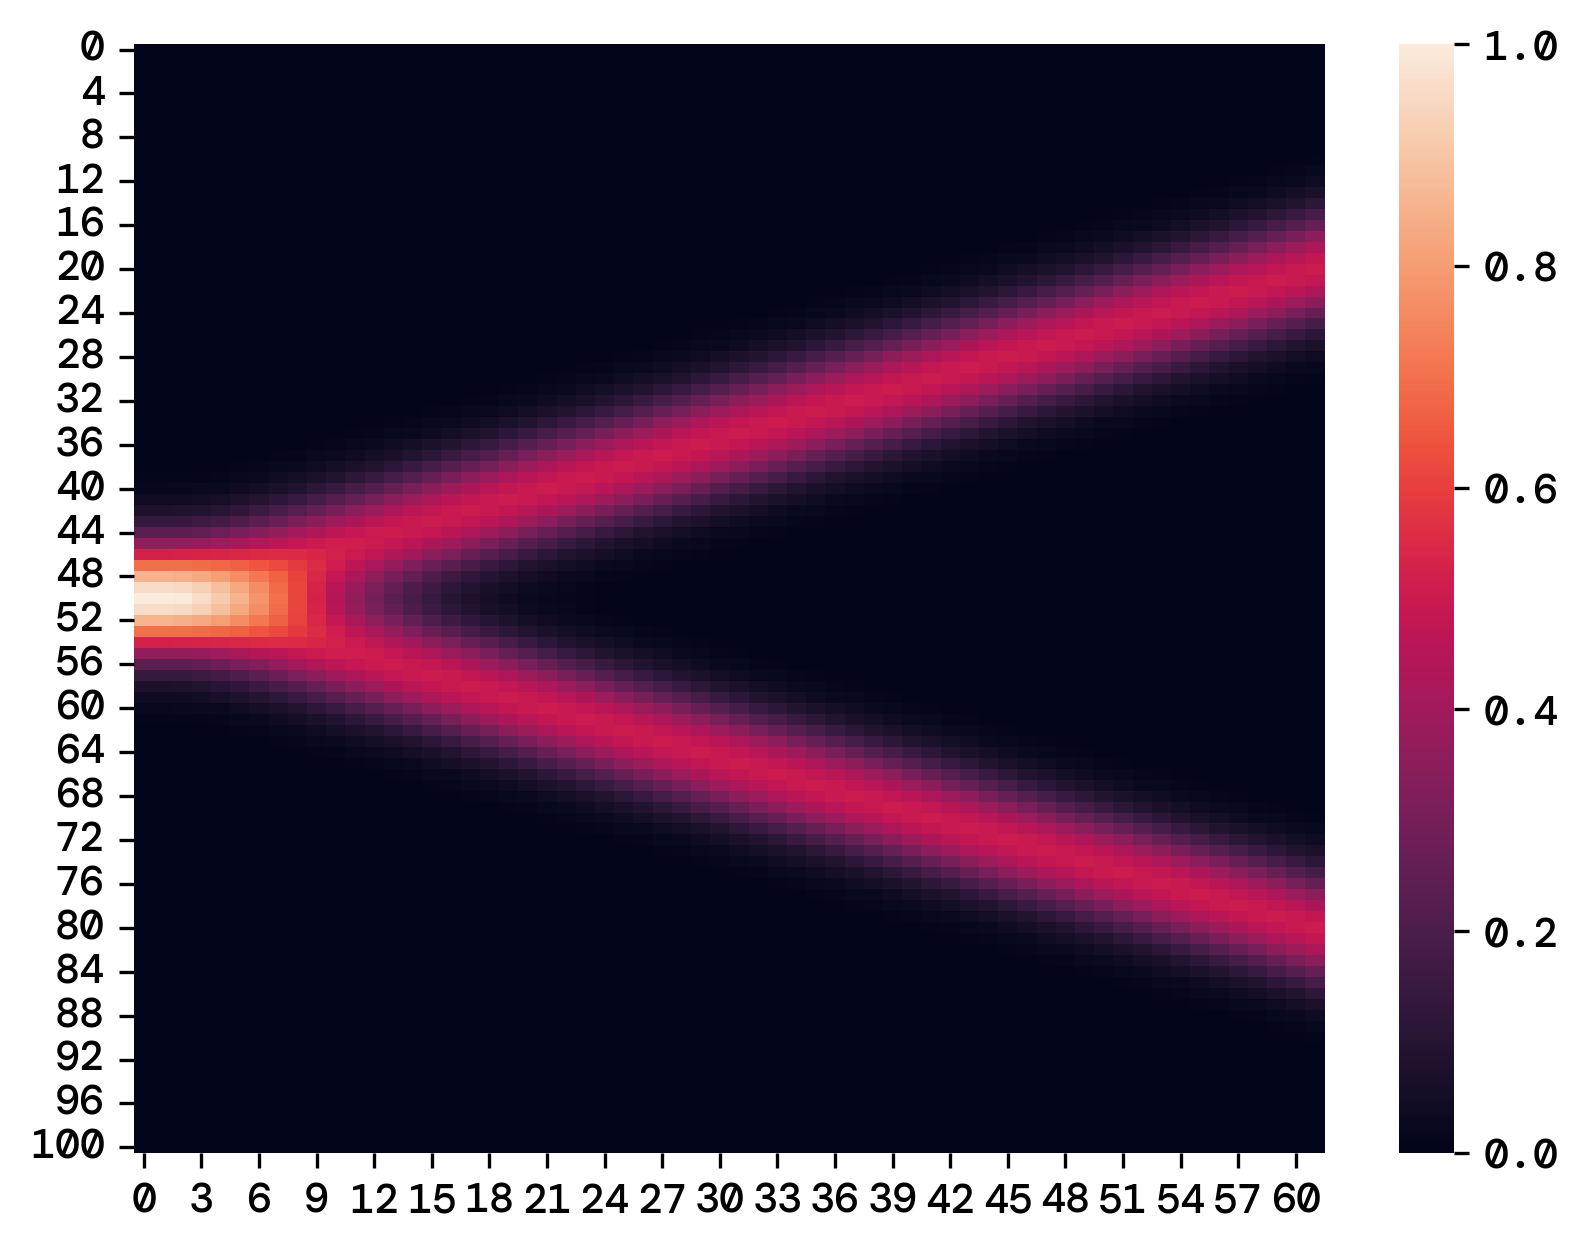
\includegraphics[width=\textwidth]{../runsAndFigures/wave_analytic.png}
            \end{center}
            \caption
            {
                Analytical solution to the wave equation.
            }\label{fig:wave_finite}
        \end{minipage}
        \hspace{2mm}
        \begin{minipage}[t]{0.5\textwidth - 1mm}
            \begin{center}
                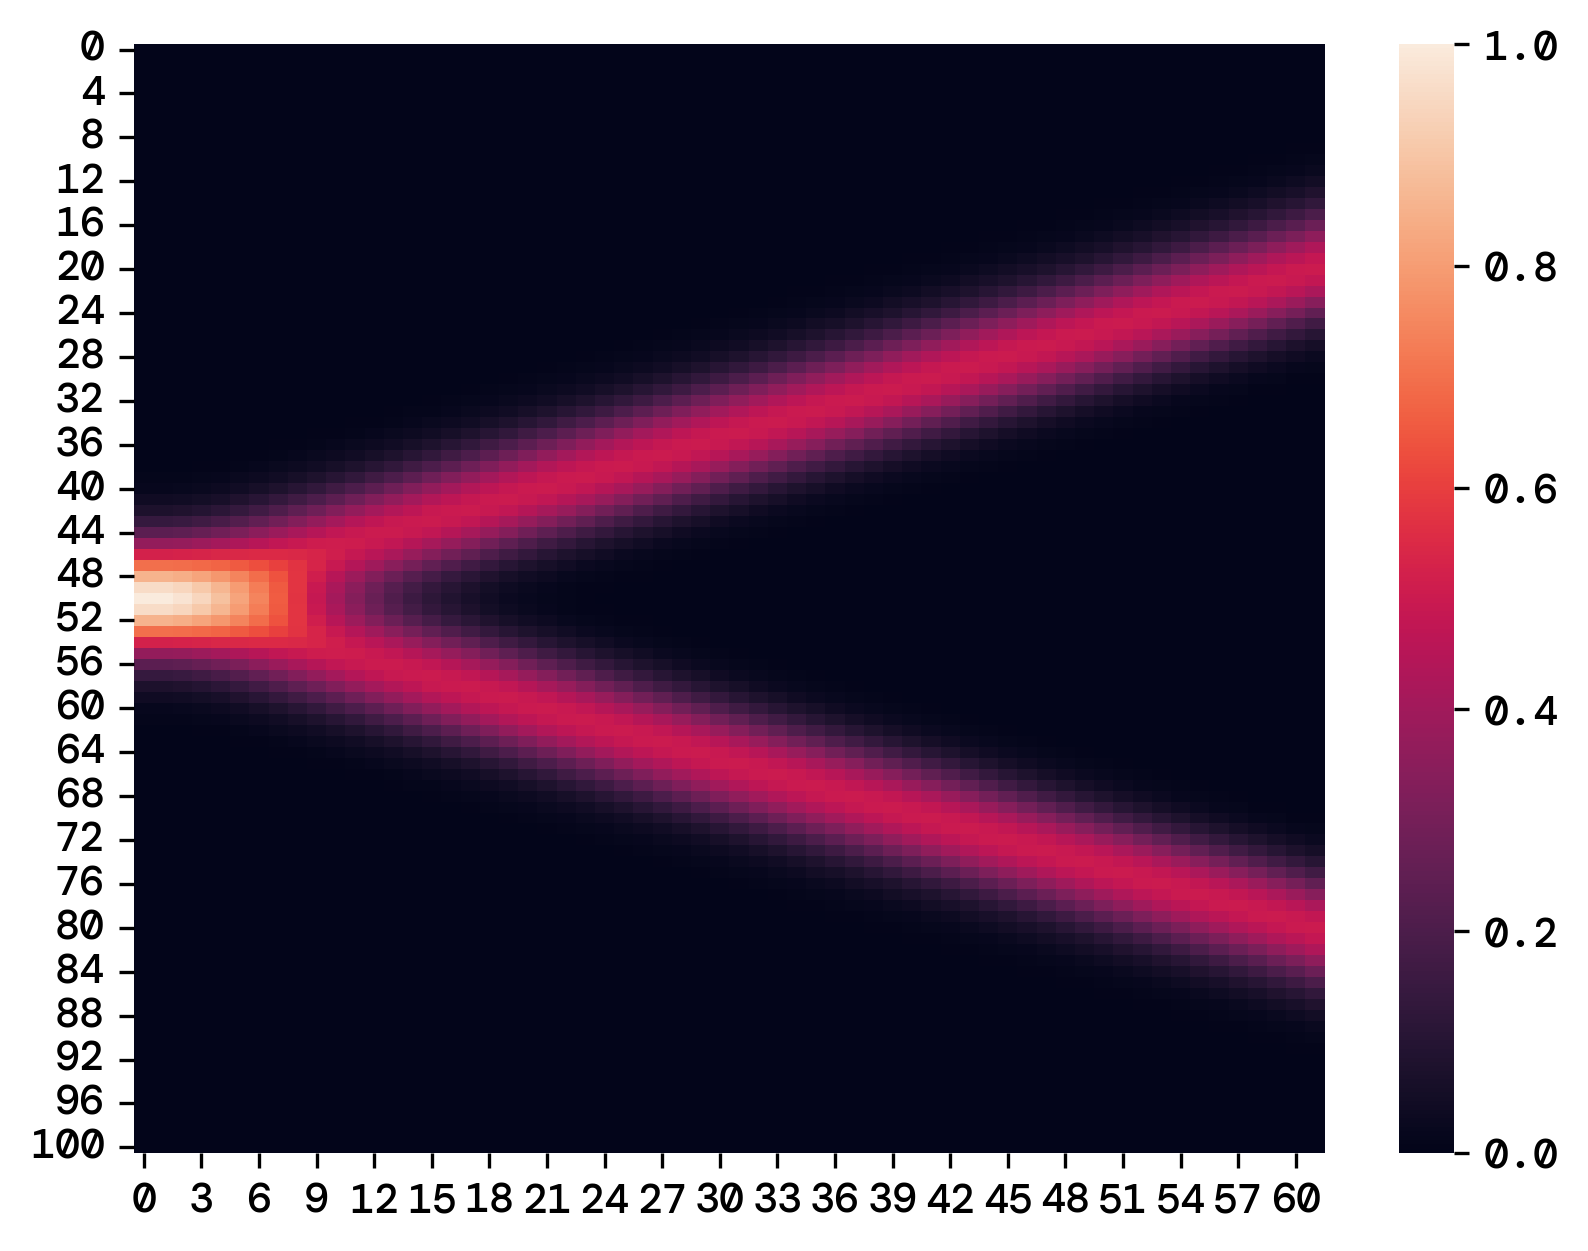
\includegraphics[width=\textwidth]{../runsAndFigures/wave_finite.png}
            \end{center}
            \caption
            {
                Finite difference solution to the wave equation.
            }\label{fig:wave_analytic}
        \end{minipage}
    \end{figure}
    \begin{figure}[!ht]
            \begin{center}
                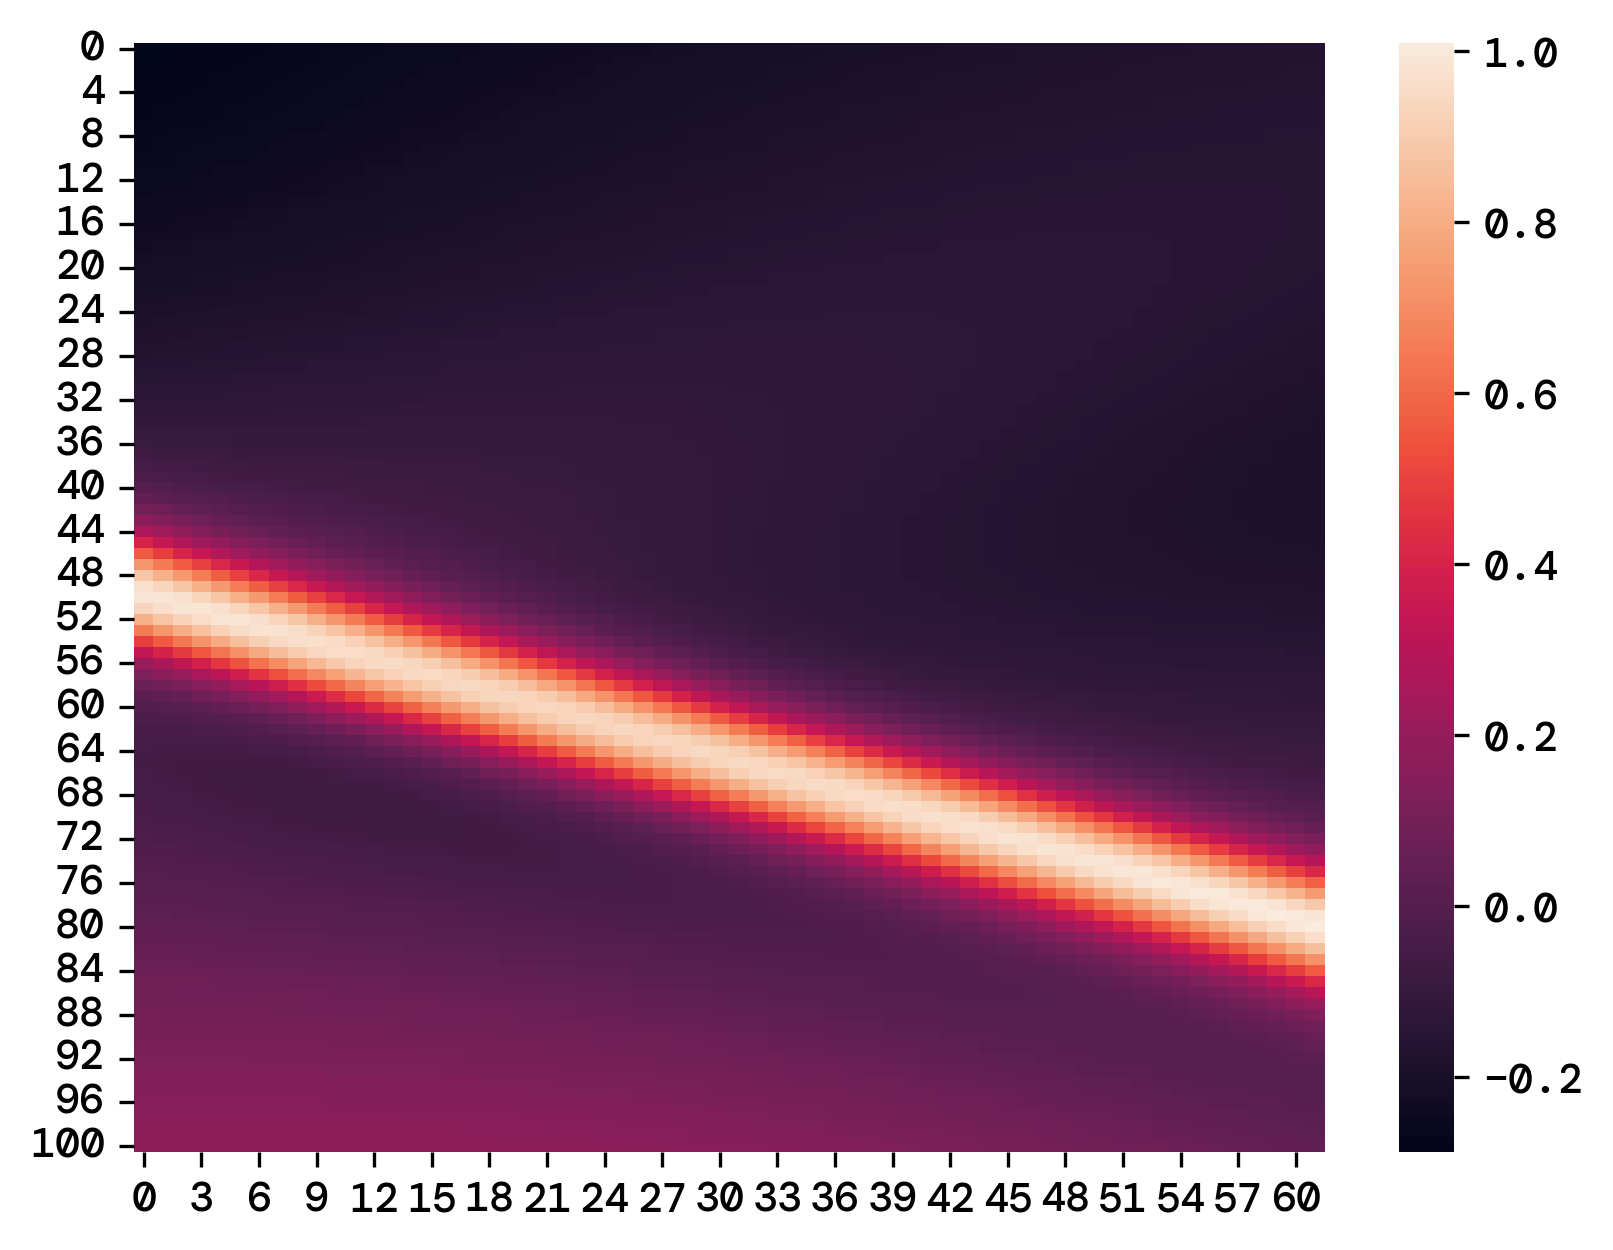
\includegraphics[width=0.5\textwidth]{../runsAndFigures/wave_tf_pinn_velocity.png}
            \end{center}
            \caption
            {
                The PINN descided to ignore the contraint on the initial momentum. Yet the solution still satisfies the
                wave equation to a certain degree.
            }\label{fig:wave_tf_dnn}
    \end{figure}

    \begin{figure}[!ht]
        \begin{minipage}[t]{0.5\textwidth - 1mm}
            \begin{center}
                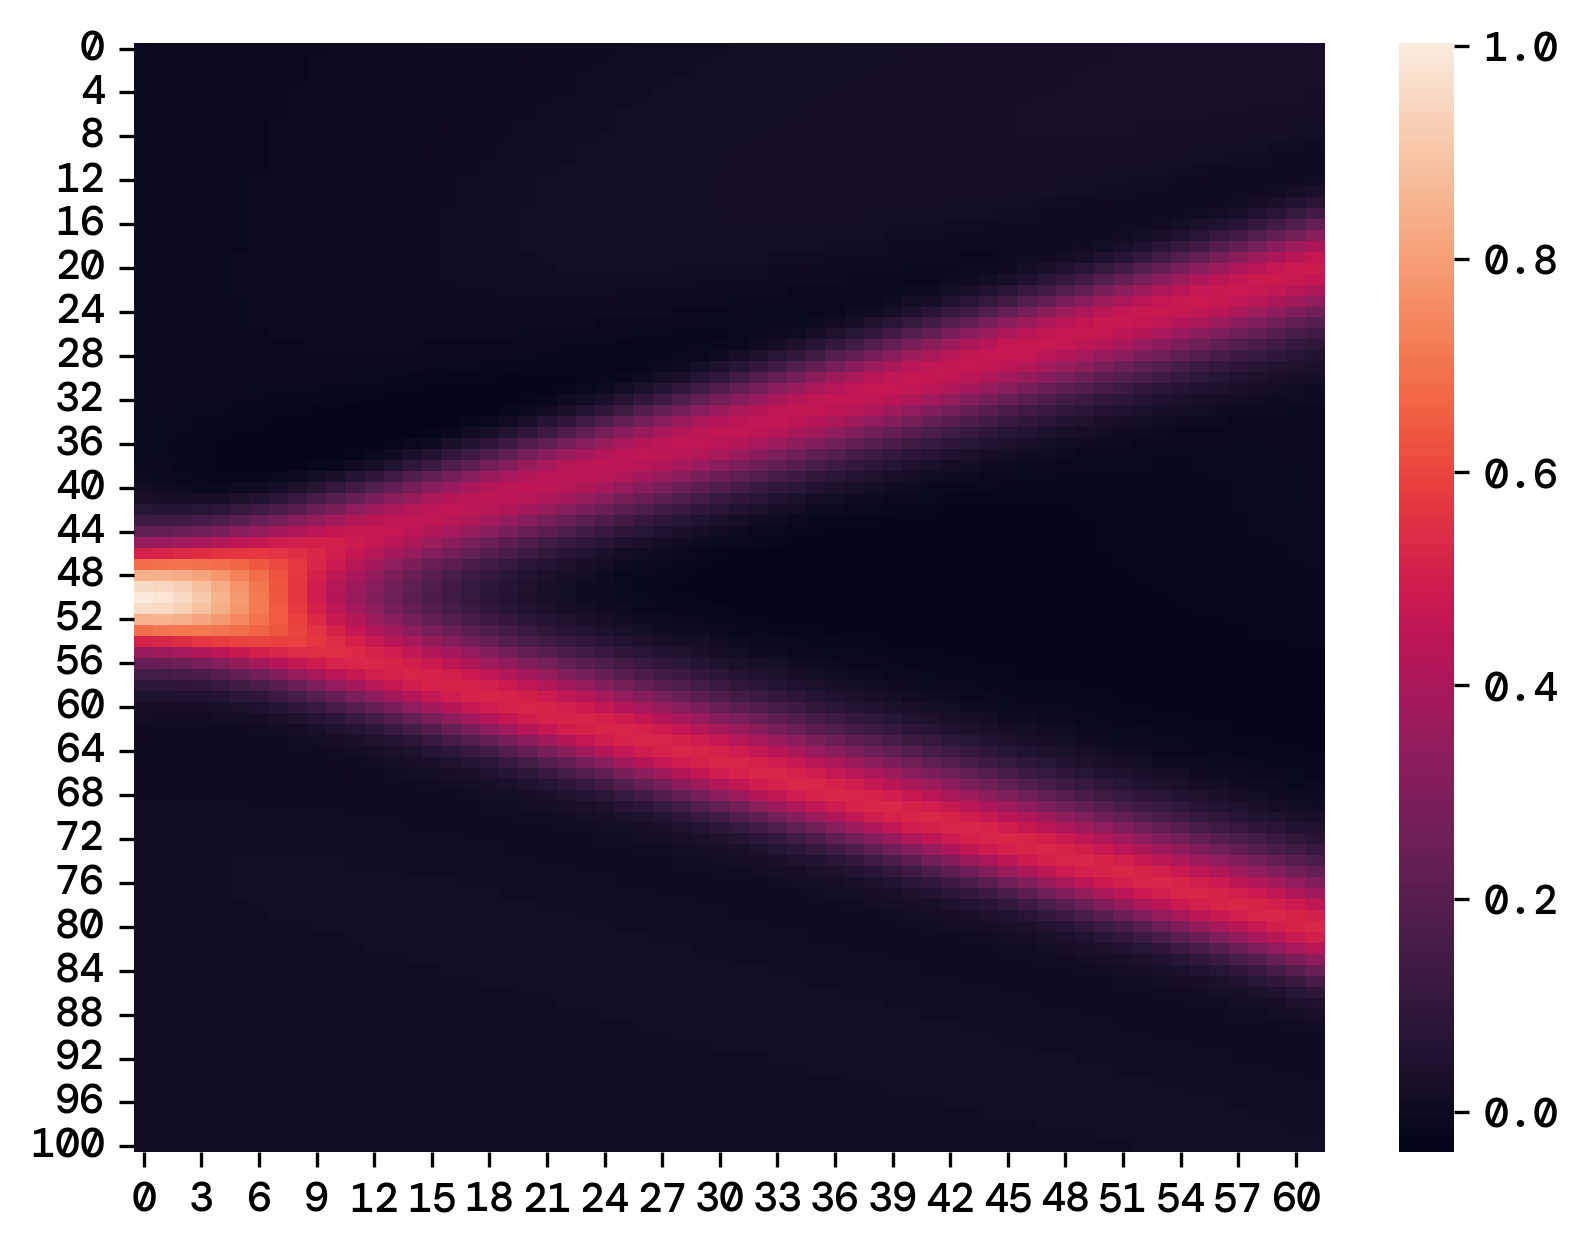
\includegraphics[width=\textwidth]{../runsAndFigures/wave_tf_hybrid.png}
            \end{center}
            \caption
            {
                The hybrid solver is able to mitigate the artifacts of the pure PINN, and is the most accurate NN solver.
            }\label{fig:wave_own_dnn}
        \end{minipage}
        \hspace{2mm}
        \begin{minipage}[t]{0.5\textwidth - 1mm}
            \begin{center}
                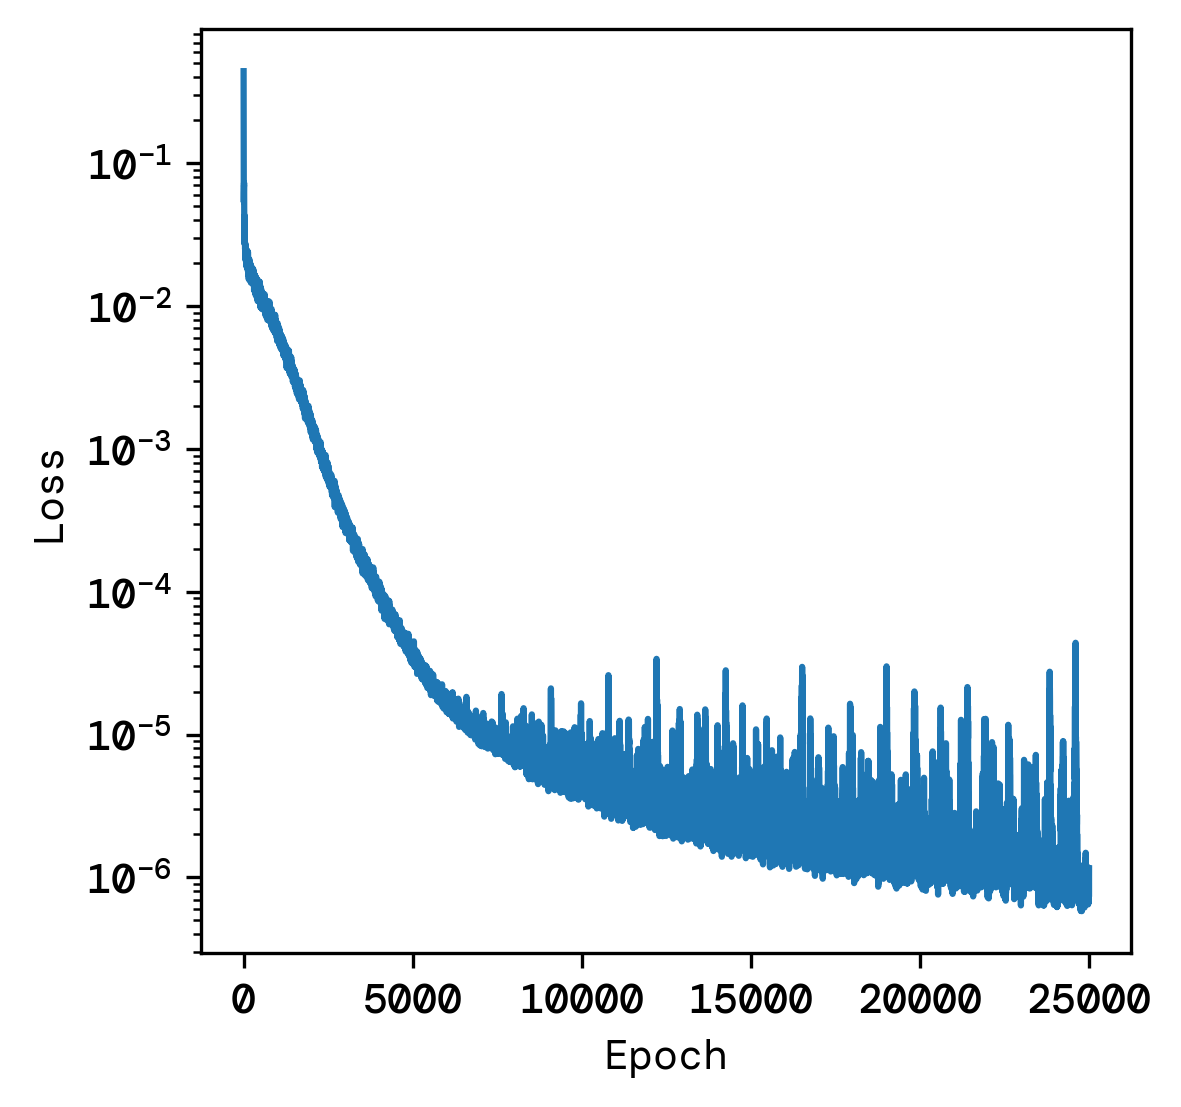
\includegraphics[width=\textwidth]{../runsAndFigures/wave_tf_hybrid_loss.png}
            \end{center}
            \caption
            {
                The PINN learns a solution to the wave equation where the initial momentum is not defined.
                Yet it satisfies the wave equation and the initial conditions.
            }\label{fig:wave_tf_dnn}
        \end{minipage}
    \end{figure}


    \begin{figure}[!ht]
        \begin{minipage}[t]{0.5\textwidth - 1mm}
            \begin{center}
                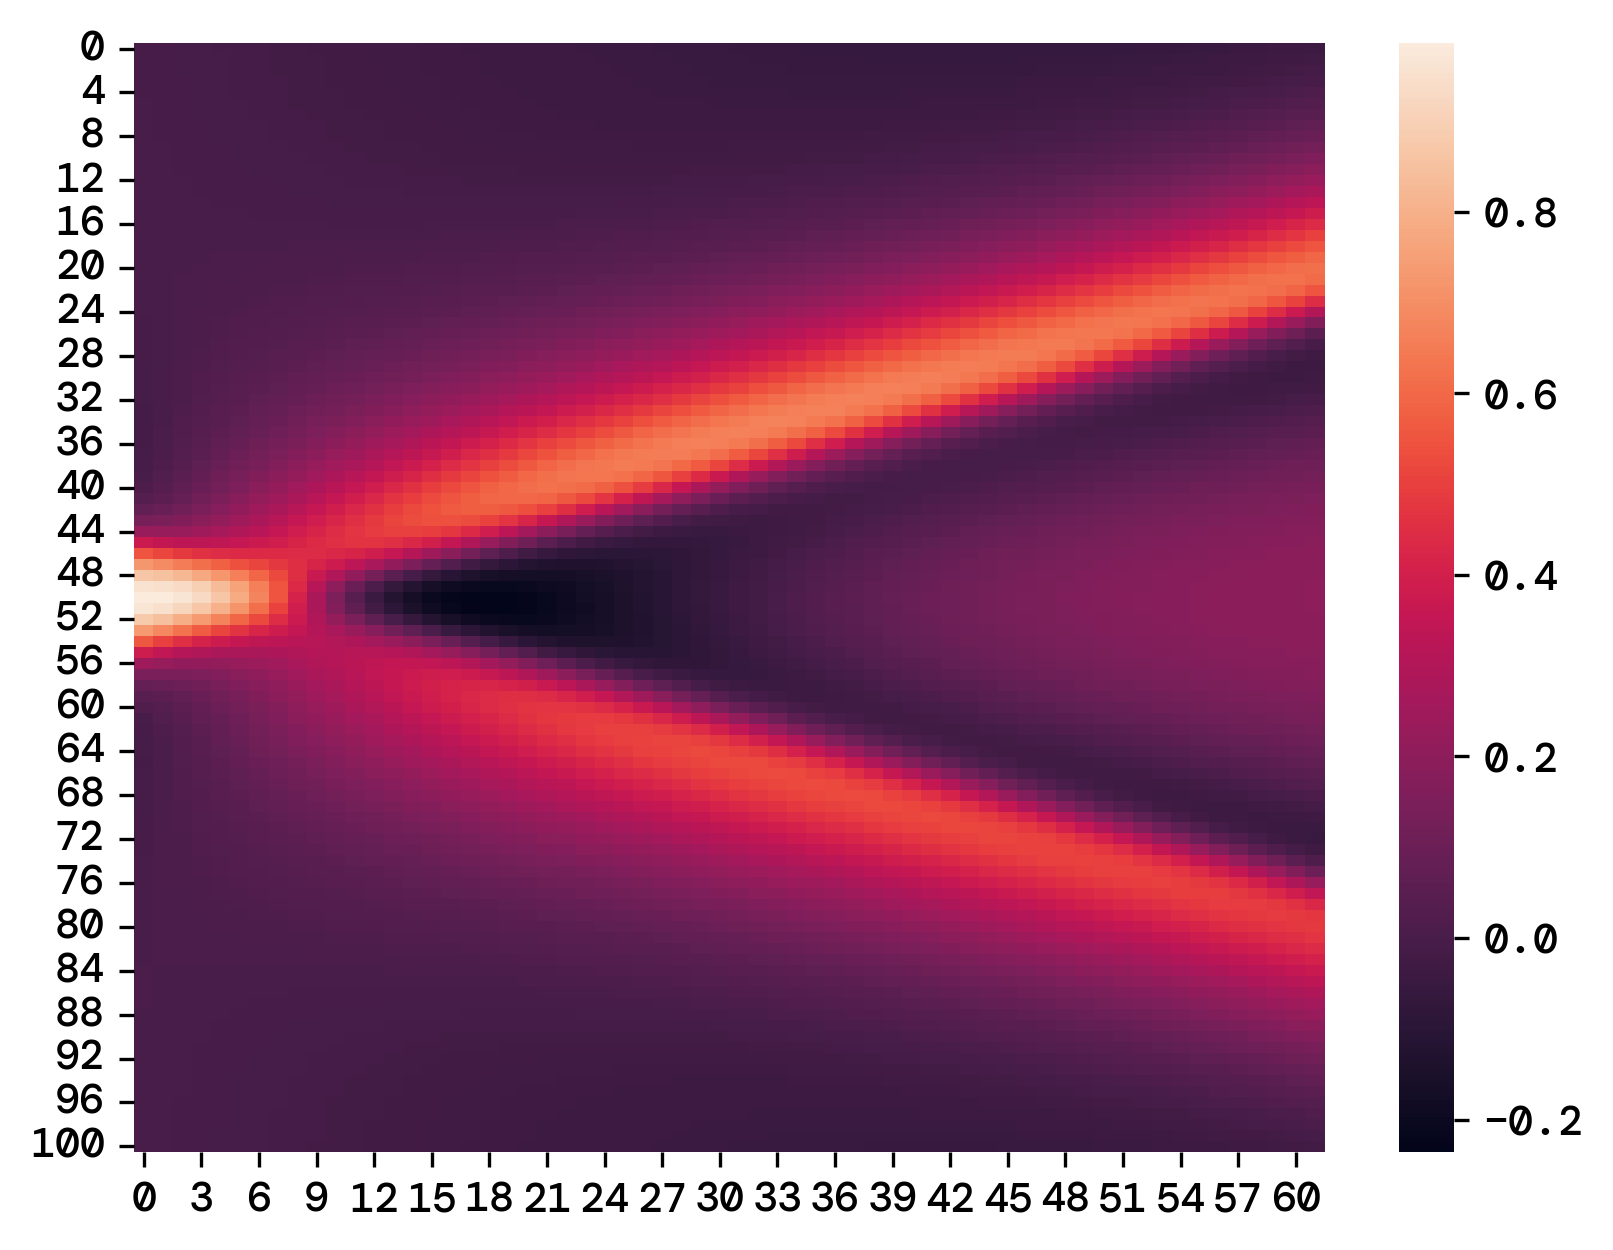
\includegraphics[width=\textwidth]{../runsAndFigures/wave_tf_pinn.png}
            \end{center}
            \caption
            {
                PINN solution to the wave equation.
            }\label{fig:wave_own_dnn}
        \end{minipage}
        \hspace{2mm}
        \begin{minipage}[t]{0.5\textwidth - 1mm}
            \begin{center}
                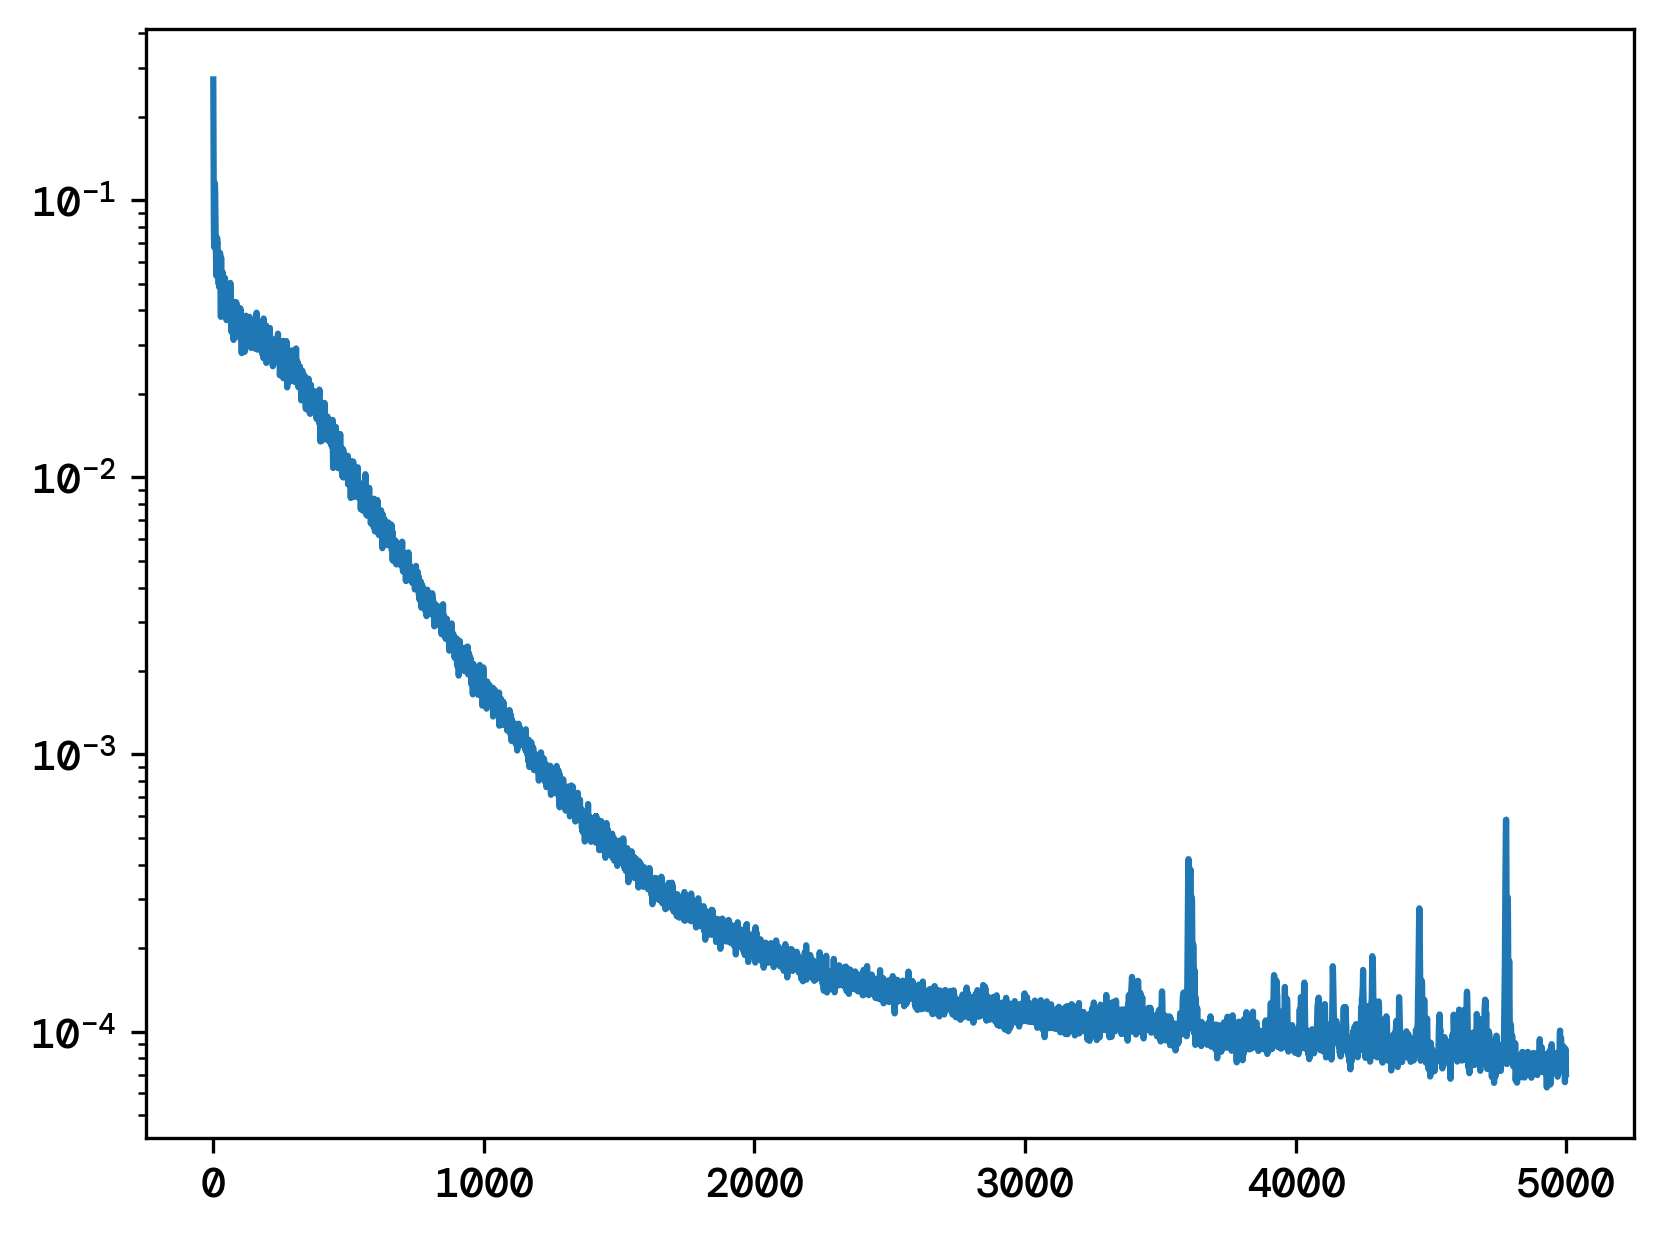
\includegraphics[width=\textwidth]{../runsAndFigures/wave_tf_pinn_loss.png}
            \end{center}
            \caption
            {
                The PINN descided to ignore the contraint on the initial momentum. Yet the solution still satisfies the
                wave equation to a certain degree.
            }\label{fig:wave_tf_dnn}
        \end{minipage}
    \end{figure}

    \begin{figure}[!ht]
        \begin{minipage}[t]{0.5\textwidth - 1mm}
            \begin{center}
                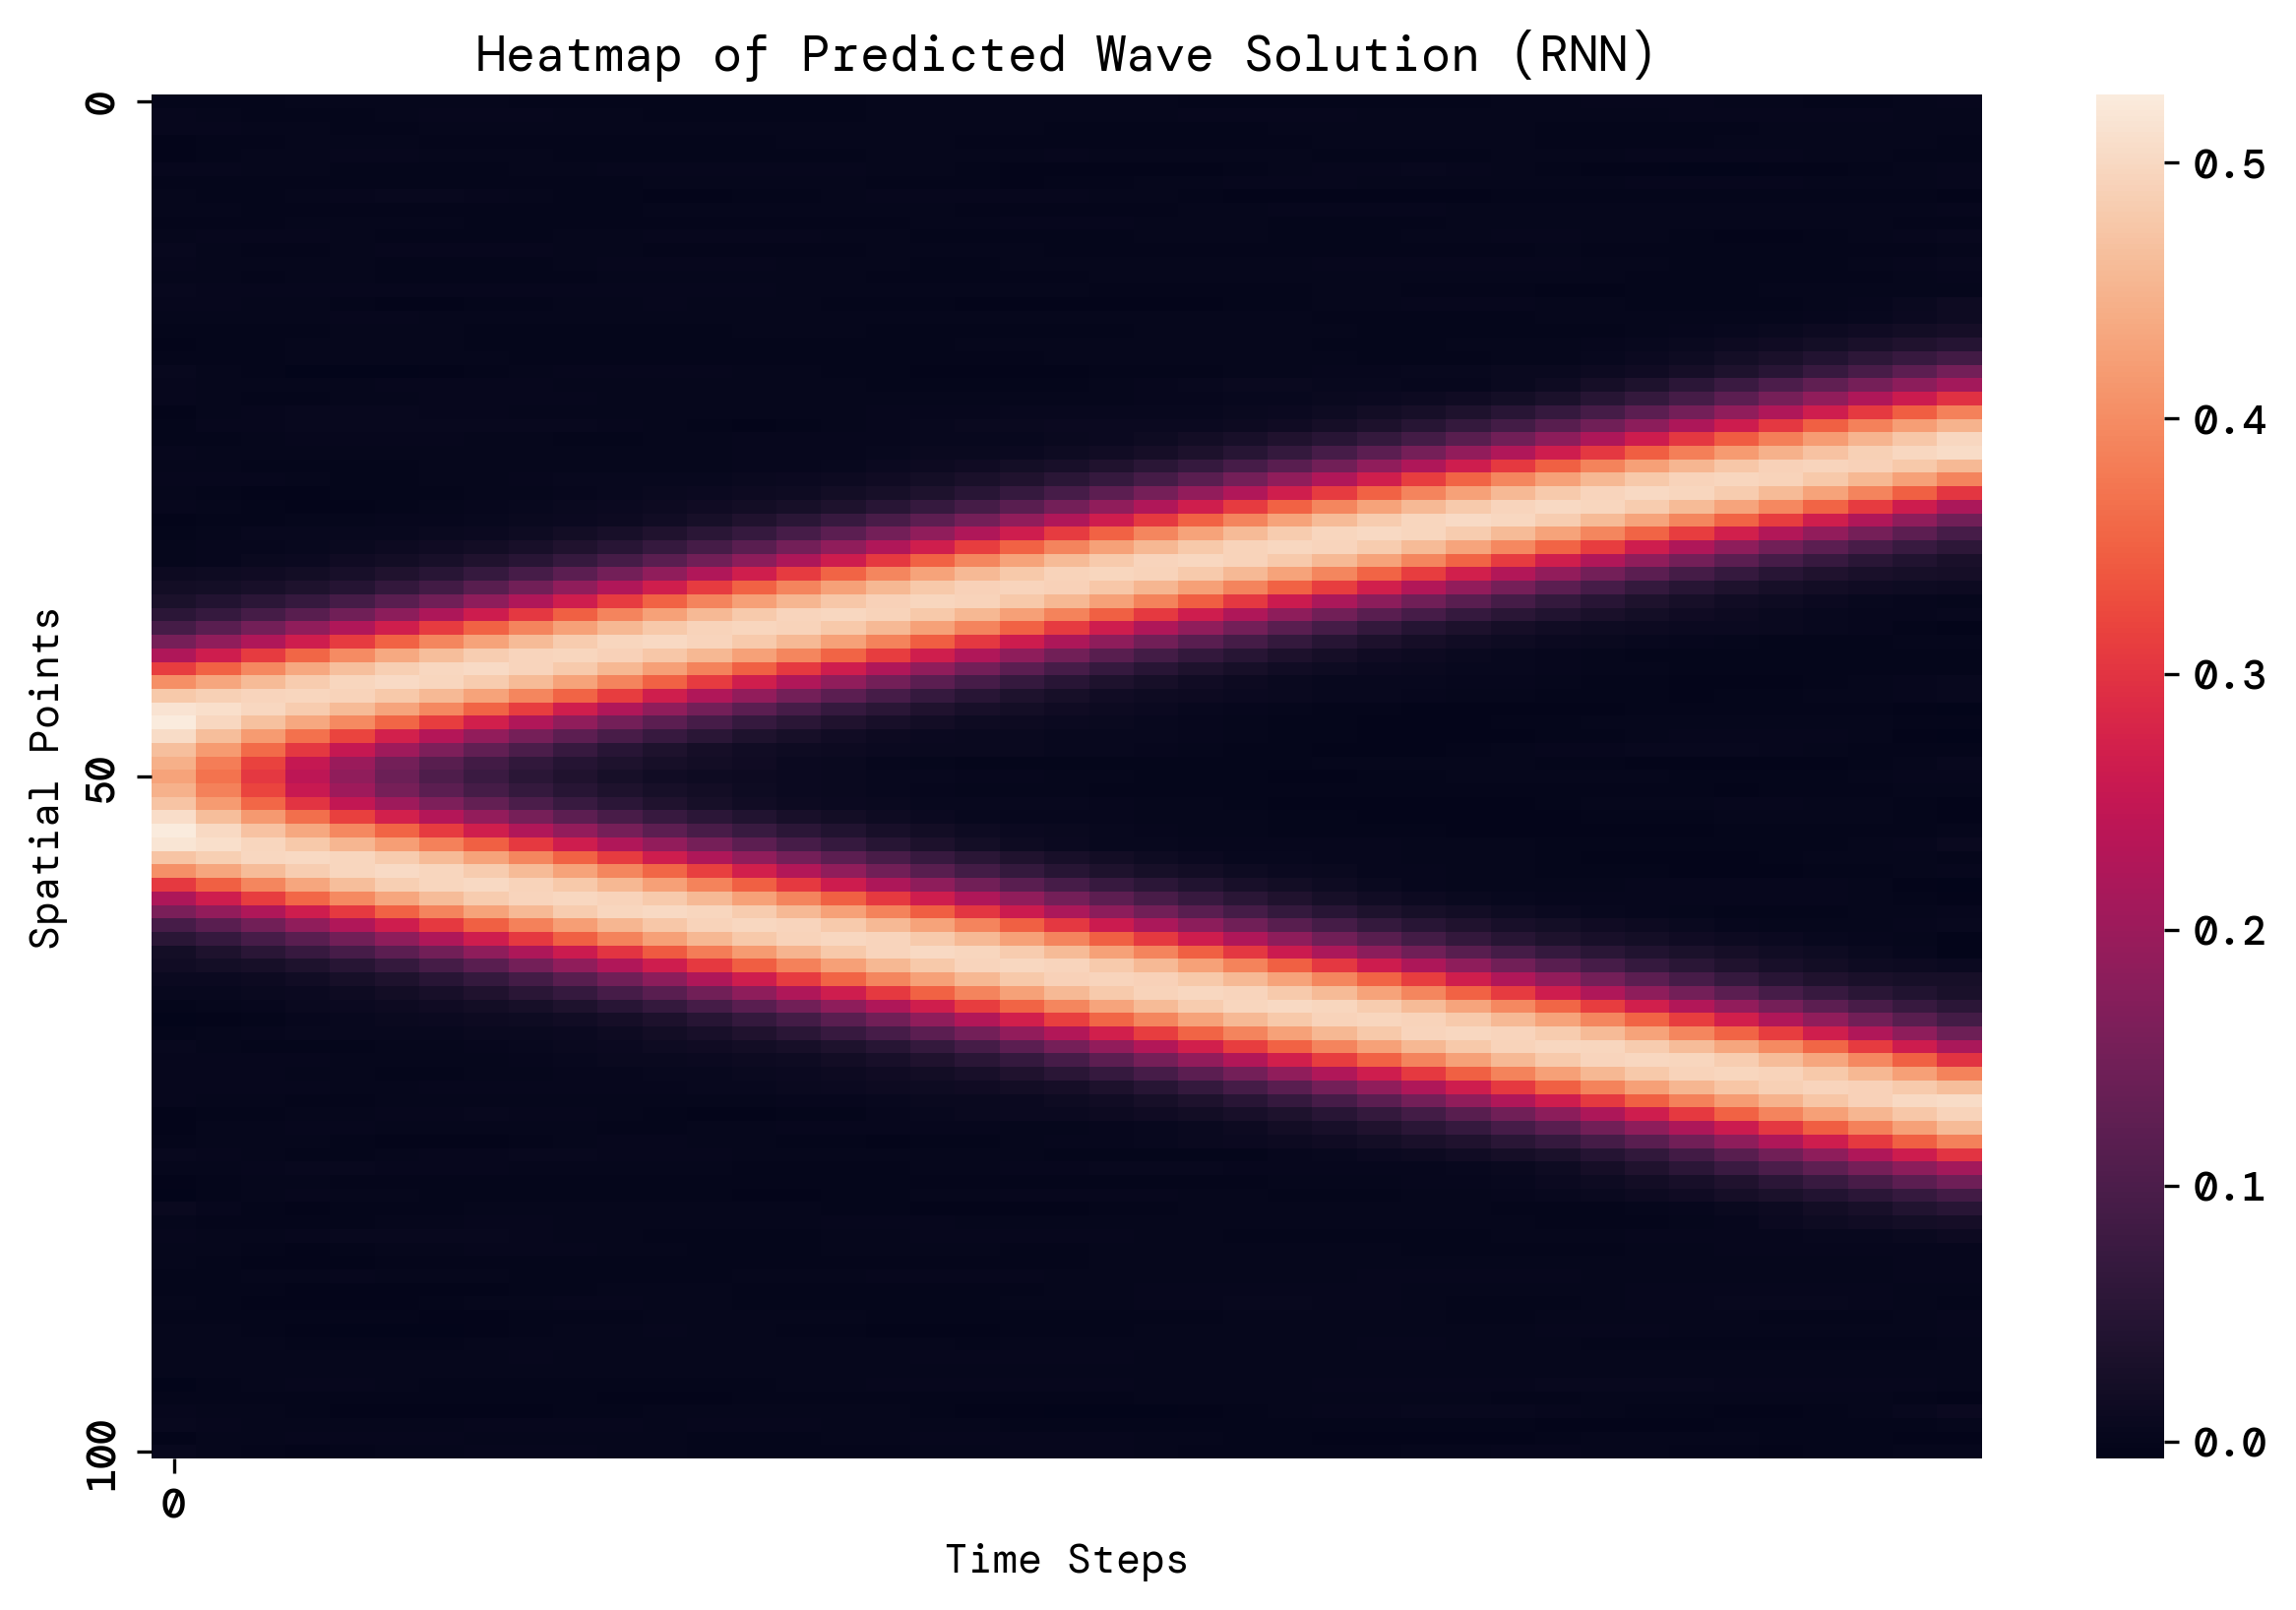
\includegraphics[width=\textwidth]{../runsAndFigures/wave_rnn.png}
            \end{center}
            \caption
            {
                PINN solution to the wave equation.
            }\label{fig:wave_own_dnn}
        \end{minipage}
        \hspace{2mm}
        \begin{minipage}[t]{0.5\textwidth - 1mm}
            \begin{center}
                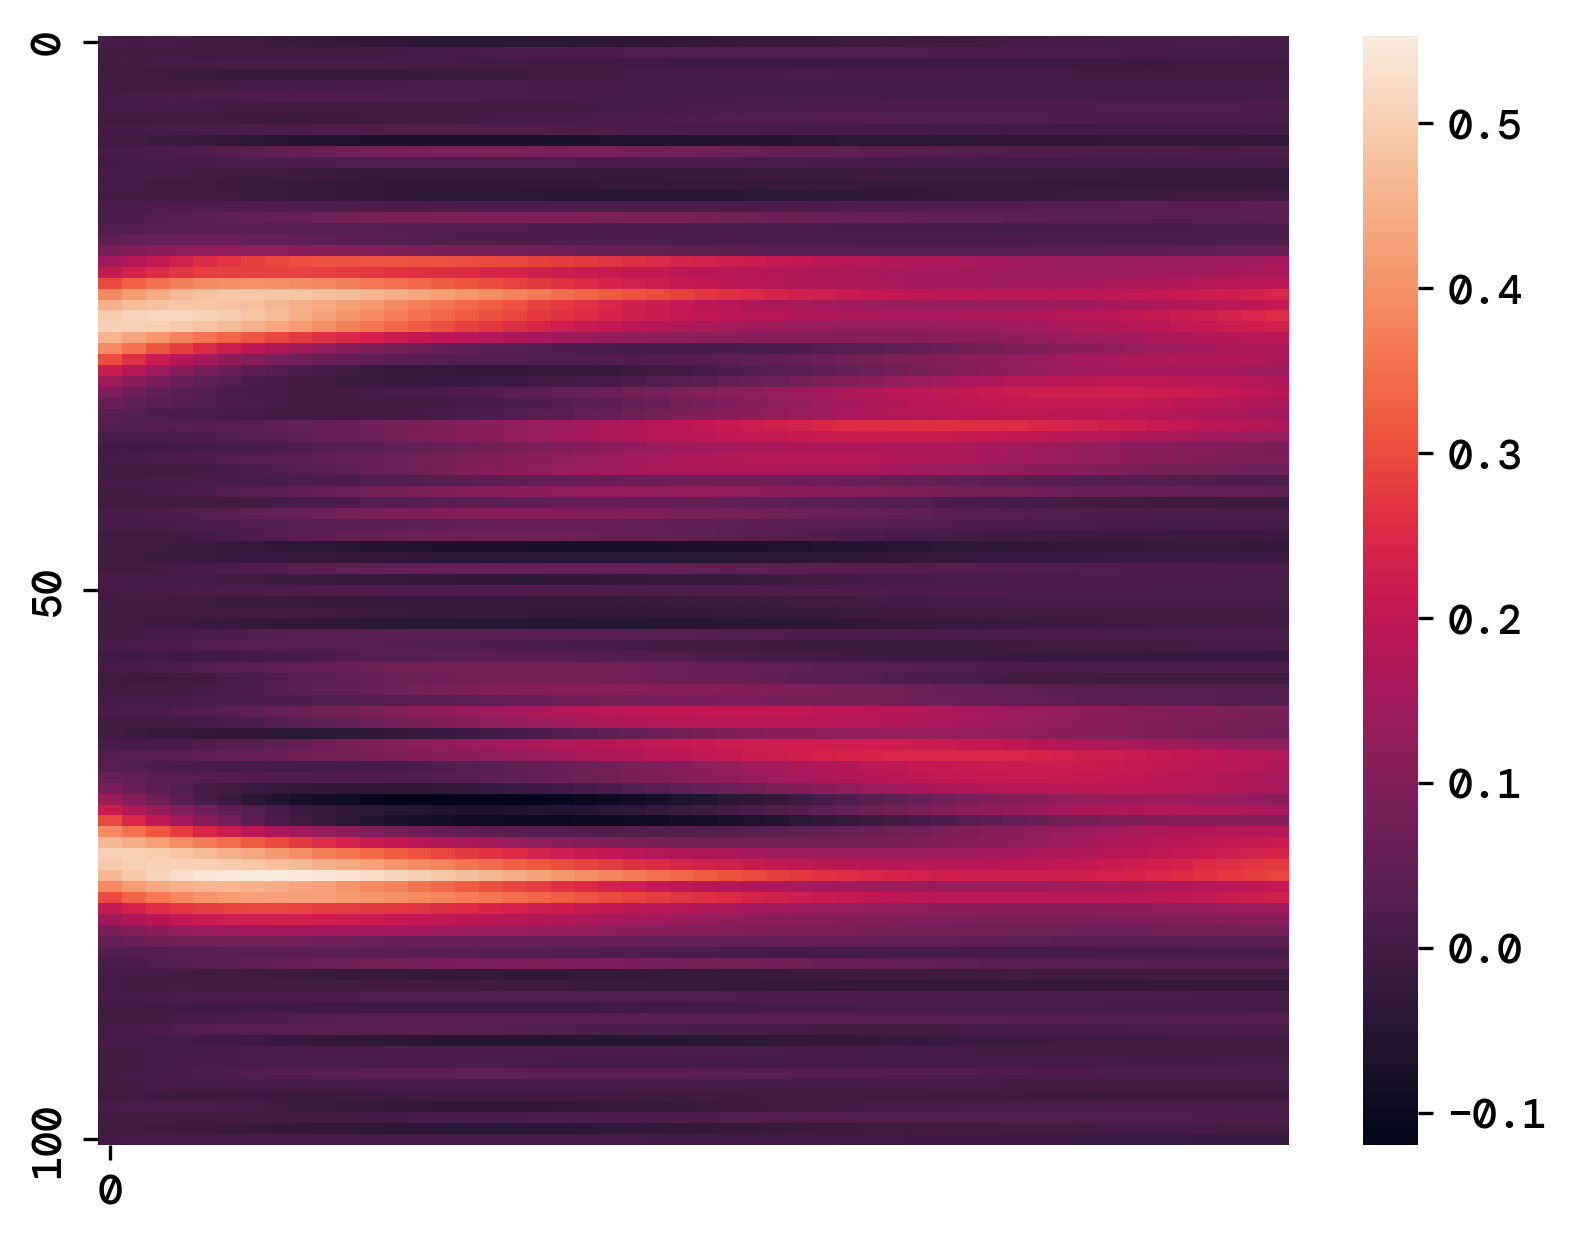
\includegraphics[width=\textwidth]{../runsAndFigures/wave_rnn_future.png}
            \end{center}
            \caption
            {
            We can see that the RNN strugles generate new data points. 
            }\label{fig:wave_tf_dnn}
        \end{minipage}
    \end{figure}



    \begin{mytable}[float=!h,label=tab:toyscores, width=0.5\textwidth]{Mean square error between 
        analytical solution and different solvers.}
    \centering
    \begin{tabular}{l|l}
        Finite difference   &\texttt{0.00855}  \\
        PINN                &\texttt{0.00879}  \\
        Hybrid              &\texttt{0.00002}  \\
    \end{tabular}%
    \end{mytable}

\subsection{Hyperparameters and Architecture}
\label{sec:hyperparameters}

    In our proof of concept, extensive hyperparameter tuning wasn't a primary focus. 
    However, we conducted preliminary experiments to understand the impact of hyperparameters 
    on model performance. Our efforts were primarily directed towards exploring how various 
    components of the loss function influence the efficiency of the hybrid solver. Notably, 
    we didn't investigate the hyperparameter effects on the RNN model's performance due to time 
    and computational resource constraints.
    For our PINN models, we implemented two hidden layers, each comprising 50 nodes. The neural 
    networks were developed using TensorFlow\cite{tensorflow2015-whitepaper}. The Adam optimizer was 
    employed with a learning 
    rate of 0.001, which provided an effective balance between computational efficiency and learning accuracy. 
    The models were trained over 10,000 epochs, using a batch size of 1,000. This approach allowed for 
    sufficient data processing while maintaining manageable computational demands. Additionally, 
    we incorporated weight decay in our training process, applying a weight of 0.0001 to prevent 
    overfitting and improve model generalization.
    The RNN model consisted of three LSTM layers, each comprising 50 nodes. The model was trained
    with the same hyperparameters as the PINN model, except for the sequence length which was set to 10.


\subsection{Comparisons}
\label{sec:comparisons}

    "paper" found that PINNs are great with better results than us
    "paper" found that RNNs are great with better results than us

    
\section{Conclusion}
\label{sec:conclusion}

    We have explored the use of neural networks in solving the wave equation. Our findings indicate that
    neural networks are capable of approximating the wave equation, although the accuracy of the models
    is not as high as we would have hoped. For our simple case where both analytical and finite difference
    solutions are available, the neural network models are not able to achieve the same accuracy. 
    However, as the partial differential equations become
    more complex, the analytical solutions may be impossible to find, and the finite difference solutions
    may become too computationally expensive or inaccurate. In these cases, neural networks may be a
    viable alternative.
    Future work could involve exploring more complex partial differential equations , such as the
    Navier-Stokes equations, with more complex bounds and initial conditions 
    and comparing the accuracy of the neural network models to the analytical
    and finite difference solutions. Another interesting direction would be to explore the use of


        Nevertheless, our experiments shed light on how loss function components can be optimized 
    to enhance the RNN model's effectiveness. This study demonstrates that a well-crafted loss 
    function can significantly influence performance, especially when it incorporates techniques 
    that leverage prior knowledge about the problem domain.
    
     








% \acks{}


% \clearpage 
%
% \appendix
% \renewcommand{\theHchapter}{appendix\Alph{chapter}}
% \renewcommand{\theHsection}{appendix\thesection}
%
% \phantomsection
% \addcontentsline{toc}{chapter}{Appendix}
%
%
% \chapter*{Appendix A}
% \label{app:appendixA}




\vskip 0.2in
\bibliography{report}
% \bibliographystyle{apalike}
\bibliographystyle{plain}
\addcontentsline{toc}{section}{Bibliography}
\end{document}

